
During this section we will be considering a canard point. This is when our fold point is shifted along the manifold - Figure \ref{fig: Canard Point}. 
\begin{figure}[h!]
	\centering
	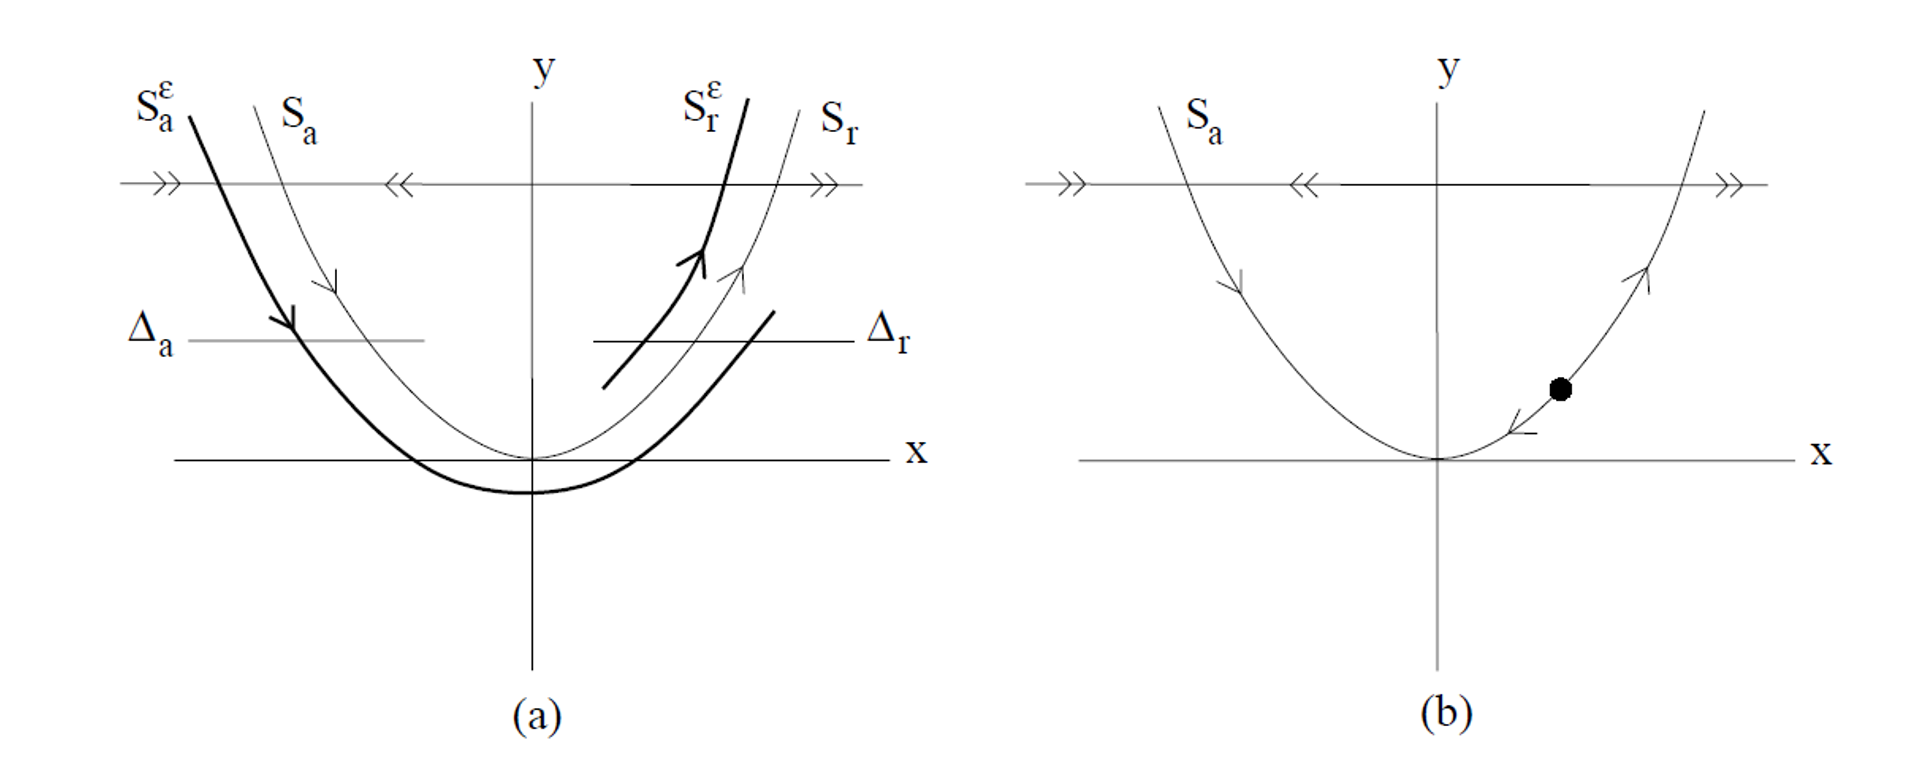
\includegraphics[height=5cm,width=8cm]{Canard_Point.png}
	\caption{The reduced flow of our system for a) $\lambda=0$ and b) $\lambda>0$.}
	\label{fig: Canard Point}
\end{figure}
To adequately explain the effect that the canard point will have on our system we will need to consider our system,
\begin{equation}
\begin{aligned}
&x'=-y+x^2-\dfrac{x^3}{3},\\
&y'=\epsilon(x-1),\\
&\epsilon'=0.\\
% &\lambda'=0,\\
\end{aligned}
\tag{\ref{eq: Fast System}}
\end{equation}
Now we need to consider Equation \ref{eq: Fast System} in terms our our cananrd system. To do this we rewrite our system with an extra parameter $\lambda$, where $\lambda$ is our perturbation of our fold point \citep{krupa2001}. \citet{krupa2001} discusses generally how we should continue with computing our canard system. If we apply his theory to the \vdp system we find,
\begin{equation}
\begin{aligned}
&x'=-y+x^2-\dfrac{x^3}{3},\\
&y'=\epsilon(x-\lambda),\\
&\epsilon'=0,\\
&\lambda'=0,\\
\end{aligned}
\label{eq: canard system}
\end{equation}
where the change in $\epsilon$ and $\lambda$ are constant. Now, for the remainder of the section, we follow the method of \citet{krupa2001} for the canard system. If we start by rewriting our canard system into the canonical forms we find,
\begin{align}
&x'=-yh_1(x,y,\epsilon,\lambda)+x^2h_2(x,y,\epsilon,\lambda),\\
&y'=\epsilon(xh_4(x,y,\epsilon,\lambda)-\lambda h_6(x,y,\epsilon,\lambda)),\\
\end{align}
Where we note that $h_j(x,y,\epsilon,\lambda)=1+O(x,y,\epsilon,\lambda)$ for $j=1,2,4,5$ and $h_3(x,y,\epsilon,\lambda)=O(x,y,\epsilon,\lambda)$. However, we should note that for the \vdp system our only term that is not solely of leading order is $h_2(x,y,\epsilon,\lambda)=1-\frac{x}{3}$. Now we are able to choose such a $\lambda>0$ that produces an equilibrium on our repelling branch $S_r$ for the reduced flow. By doing this we are then able to define the following conditions for our reduced flow on $h_j$,
\begin{align}
&a_3=\pd{}{x}h_2(0,0,0,0)=-\frac{1}{3},\\
&A=-a_2+3a_3-(2a_4+2a_5)=-1,
\end{align}
where we notice that our other solutions for $a_i=0$ for $i=1,2,4,5$ are trivial. The reason that we consider the constant $A$ is because we will find that this constant is crucial in our canard point analysis iff $A\neq 0$ \citep{krupa2001}. Following this \citep{krupa2001} discusses the existence of a critical value for $\lambda$ (denoted $\lambda_c$), where our two branches $S_r$ and $S_a$ must connect in a smooth fashion. Now from \textit{Theorem 3.1} we nkow that we must have a transition map at our critical point,
\begin{equation}
\lambda_c(\sqrt{\epsilon})=-\epsilon(\frac{a_1+a_5}{2}+\frac{A}{8})+O(\epsilon^\frac{3}{2}),
\end{equation}
which can be written as $\lambda_c(\sqrt{\epsilon})=\frac{\epsilon}{8}+O(\epsilon^\frac{3}{2})$ for the \vdp system \citep{krupa2001}. Consider Canard cycles and center manifolds / Freddy Dumortier, Robert Roussarie. for more details on canards in \vdp.


\subsection{Canard Blow-up}
Now similarly to Section \ref{sec: VDP Blowup} we consider various transformations of our coordinate system to be able to be able to consider the non-hyperbolic equilibrium induced by our canard point. However, as we would expect with our new system we should consider a new set of transformations \citep{krupa2001}.
\begin{equation}
x=\bar{r}\bar{x}, \ y=\bar{r}^2y, \ \epsilon=\bar{r}^2\bar{\epsilon}, \ \lambda=\bar{r}\bar{\lambda}
\end{equation}
Now that we have established the transformation we can then define our transformations for $K_1$ and $K_2$ but it is not necessary to consider the third chart ($K_3$). This is because we find that the attracting slow manifold connects to the repelling slow manifold. As a result of this we find that our flow will `bend back' from $K_2$ into $K_1$ instead of flowing out into the fast flow, which is described by $K_3$. This concept can be described by the Figure \ref{fig: flow in canard}.
\begin{figure}[h!]
	\centering
	%    \includegraphics{}
	\caption{Figure describing canard flow in manifold}
	\label{fig: flow in canard}
\end{figure}


Since we have established why we need only consider two charts we can our transformations,
\begin{subequations}
	\begin{align}
	&x=r_1x_1, \ y=r_1^2, \ \epsilon=r_1^2\epsilon_1, \ \lambda=r_1\lambda_1 \label{eq: coordiante K_1}\\ 
	&x=r_2x_2, \ y=r_2^2y_2, \ \epsilon=r^2_2, \ \lambda=r_2\lambda_2 \label{eq: coordinate K_2}
	\end{align}
\end{subequations}
Since these transformations have been defined we should consider our charts. We will first consider chart 2, for analogous reasoning to Section \ref{sec: VDP K_2}. 

\subsubsection{Dynamics in \texorpdfstring{$K_2$}{K2}}
We start by noting that we are considering our invariant plane at $r_2=0$ which will significantly simplify our system for $K_2$. Further we should note that we are taking a transformation in time, $\od{r}{t_2}=\od{t}{t_2}\od{r}{t}=\frac{1}{r_2}\od{r_2}{t}$, as well as in our coordinates. Then if we substitute our time transformation and Equation  \ref{eq: coordinate K_2} into our system of Equations \ref{eq: canard system} we find, 
\begin{subequations}
	\begin{align}
	r_2^2x_2' - r_2x_2r_2'&=-r_2^2y_2h_1+r^2_2x^2_2h_2,\notag\\
	\implies x'_2&=-y_2+x_2^2-r_2G_2(x_2,y_2),\\
	%     \end{aligned}
	% \end{equation*}
	% \begin{equation}
	%     \begin{aligned}
	r^3_2y_2'-3r_2^2y_2r_2'&=r^2_2(r_2x_2h_4-r_2\lambda_2h_5),\notag\\
	\implies y_2'&=x_2-\lambda_2+r_2G_2(x_2,y_2), \label{eq: K_2 y trans}
	\end{align}
	\label{eq: reduced canard k_2}
\end{subequations}
where we note that $h_j=h_j(x,y,\epsilon,\lambda)$ for $j=1,2,3,4,5$. We should also recall that $r_2'=\lambda_2'=0$. Notice that we have included an additional term in Equation \ref{eq: K_2 y trans} - we define $G_2(x_2,y_2)$ in the following way, $G(x_2,y_2)=(G_1(x_1,y_1),G_2(x_2,y_2))^T=(-\frac{x^2_2}{3},0)^T$. The reason we also define this vector is to aide in the Melnikov computations which we will see later. \citet{krupa2001} discusses that for this chart we have an interesting result. They note that at $r_2=\lambda_2=0$ our system is integrable which allows us to define a constant of motion $H(x_2,y_2)=\frac{1}{2}\exp{(-2y_2)}\left(y_2-x^2_2+\frac{1}{2}\right)$ which we can easily verify \citep{krupa2001} using the following equations,
\begin{align*}
x'_2&=e^{2y_2}\pd{H}{y_2}(x_2,y_2),\\
y_2'&=-e^{2y_2}\pd{H}{x_2}(x_2,y_2).
\end{align*}
Further to this we can see, when we consider our reduced system, that we have an equilibrium at the origin, implying that $H(x_2,y_2)=h$.
considering the reduced system (Equation \ref{eq: reduced canard k_2}) we find from $ H(x_2,y_2)=0 $ that,
\begin{subequations}
	\begin{align}
	x_2'&=\frac{1}{2}\ \	\implies x_2=\frac{t_2}{2}+A, \label{canard: trajectory x}\\
	y_2'&=\frac{t_2}{2}\ \implies y_2=\frac{t_2^2}{4}-\frac{1}{2}, \label{canard: trajectory y}
	\end{align}
\end{subequations} 
where we have directly integrated Equation \ref{canard: trajectory x} with respect to our time ($ t_2 $). However, we can note that we are able to choose $ A=0 $ as we are considering an autonomous (time-invariant) system. Then for Equation \ref{canard: trajectory y} we are able to rearrange constant of motion at zero to give, $ y_2=x_2^2-\frac{1}{2} $. Clearly from this analysis we are then able to define our trajectories in terms of $ \gamma_{c,2} $, 
\begin{equation}
\gamma_{c,2}(t_2)=(x_{c,2}(t_2),y_{c,2}(t_2))=\left(\frac{t_2}{2},\frac{t^2_2}{4}-\frac{1}{2}\right).   
\end{equation}
Now that we have established that we must have a flow on our second chart, then there must also exist transition maps. Therefore this now enables us to consider the first chart in the following section.


\subsection{Dynamics in \texorpdfstring{$K_1$}{K1}}
For $K_1$ we follow a similar approach to the above. We will use the transformations, 
\begin{equation}
x=r_1x_1, \ y=r_1^2, \ \epsilon=r_1^2\epsilon_1, \ \lambda=r_1\lambda_1 \tag{\ref{eq: coordiante K_1}},
\end{equation}
to find the relevant pathways of our flows. Now if we first consider the $r_1$ component, 
\begin{align}
2r_1^2r_1'=r_1^2\epsilon(r_1x_1-r_1\lambda_1), \label{canard: r_1}
\end{align}
where we can call $F=F(x,y,\epsilon,\lambda)=x_1-\lambda_1+O(r_1(r_1+\lambda_1)$. Now we will see the motivation with starting with $y=r_1$ when we transform our other coordinates. Now if we consider $x=r_1x_1$,
\begin{align*}
r_1r_1'x_1+r_1^2x_1'&=-r_1^2+r_1^2x_1^2,\\
x_1'&=-1+x_1^2-\frac{x_1r_1'}{r_1},
\end{align*}
where we can use Equation \ref{canard: r_1} to simplify this further - Equation \ref{eq: canard x_1}.
\begin{align}
x_1'=-1+x_1^2-\frac{x_1}{r_1}\left(\frac{r_1\epsilon_1F}{2}\right) \label{eq: canard x_1}
\end{align}
We now consider our $\epsilon=\epsilon_1r_1^2$ and noting $\epsilon'=0$. Then we have, $r_1^3\epsilon'=-2r_1^2\epsilon_1r_1'$, where we can use Equation \ref{canard: r_1} to simplify to,
\begin{align}
\epsilon'=-\epsilon_1^2F. \label{canard: epsilon k_1}
\end{align}
Our last transformation is for our new coordinate $\lambda=r_1\lambda$, noting that $\lambda'=0$. Similarly to the above we find $r_1^2\lambda_1'+r_1\lambda_1r_1'=0$ then, 
\begin{equation}
\lambda'_1=-\frac{\lambda_1\epsilon_1F}{2}, 
\end{equation}
which is a trivial rearrangement as seen in Equation \ref{canard: epsilon k_1}. Now if we combine the above we find that our transformed system is of the following form,
\begin{subequations}
	\begin{align}
	r_1'&=\frac{\epsilon}{2}(r_1x_1-r_1\lambda_1), \\
	% \label{canard: r_1}
	x_1'&=-1+x_1^2-\frac{x_1\epsilon_1F}{2},\\
	\epsilon'&=-\epsilon_1^2F,\\
	\lambda'_1&=-\frac{\lambda_1\epsilon_1F}{2}.
	\end{align}
	\label{canard: system of equations}
\end{subequations}
% Unique becuase of exponetial attraction in canard case - note it is the reversal of figure 2.4 for uniqueness
From this system we are now able to make some deductions. We first can observe that the hyperplanes are along the $r_1=\epsilon_1=\lambda_1=0$ with an invariant line at $l_1=\{(x_1,0,0,0): x_1\in\Re\}$ \citep{krupa2001}. As \citet{krupa2001} discusses the equilibria present at the end of both of our branches - Figure \ref{fig: Canard Point} - which are found at $p_a=(-1,0,0,0) \ \text{and} \ p_r=(1,0,0,0)$ \citep{krupa2001}. Now we can go one step further, we can consider Equation \ref{canard: system of equations} and find the eigenvalues of the system for the invariant planes. We find that, 
\begin{equation}
J-\lambda I= \begin{bmatrix}
2x-\lambda & 0 & 0 & 0  \\
0 & -\lambda & 0 & 0&\\
0 & 0 & -\lambda & 0 \\
0 & 0 & 0 & -\lambda
\end{bmatrix},
\end{equation}
which clearly has three zero eigenvalues and one non-zero eigenvalue $\lambda=\pm 2$. Which further empahsises that our equilibrium point is non-hyperbolic. As a result we intuitively expect that something interesting occurs at this point. In the section following we will be considering what effect these mappings and eigenvalues will have on our system.

\subsubsection{Separation of the Manifolds}

\textbf{Discuss splitting on the manifold}

\subsection{Effect of the Canard Point}\label{sec:effect-of-the-canard-point}
Now that we have shown that there must exist a flow around our fold point we should now consider the global effect of the canard point. We can see by considering the  system of Equations \ref{canard: system of equations} that our equilibriums are at $ (x,y)=(\lambda,\lambda^2[\frac{1-\lambda}{3}]) $ and find the eigenvalues from the matrix, 
\begin{equation}
A-\mu I=\begin{bmatrix}
2x-x^2-\mu&-1&0&0\\
0&-\mu&0&0\\
0&0&-\mu&0\\
0&0&0&-\mu
\end{bmatrix}.
\end{equation}
\textbf{Then our eigenvalues are, $ \mu=(2-x)x \ \text{and} \ \mu=0 $, noting that we have an upper triangular matrix. Then we can note that we have a complex eignevalue which causes a Hopf bifurcation, as shown below:}%wrong maths

From the following Figures we can see the pregression of our flow over the system,
\begin{figure}[h!]\centering
	\includegraphics[]{}
	\caption{Development of the Hopf Bifurcation.}
	\label{fig: Hopf}
\end{figure}, 
which we can see that we have an unstable periodic solution within our canard system. \textbf{We can also further deduce from this calculation that we have an amplitude of $ O() $} \citep{krupa2001}.


\subsubsection{Singular Hopf Bifurcation}
In this section we will further expand on our Hopf Bifurcation of the previous section (Section \ref{sec:effect-of-the-canard-point}). We note that we get a singular bifurcation iff our system is equivalent to Equation \ref{eq: Fast System}, \st $ \lambda=1 $. \citet{Eckhaus} discusses that our bifuraction will only exist within a small range of $ O(\epsilon) $. Then to model this behaviour we need to consider a small perturbation along the slow flow where we will have, from Equation \ref{eq: canard system},
\begin{equation}
\dot{y}=\lambda-x+\nu y,
\end{equation}
where $ \nu $ is of order $ O(\epsilon) $, thus small. We can immediately see that when $ \nu=0 $ that we have our orignal flow at our equilbrium but we are now able to perturb our flow over a small domain, which are described in Figures \ref{fig: Hopf}. We can also see how our system behaves when our $ \nu $ is of larger order than $ O(\epsilon) $,

\begin{figure}[h!]\centering
	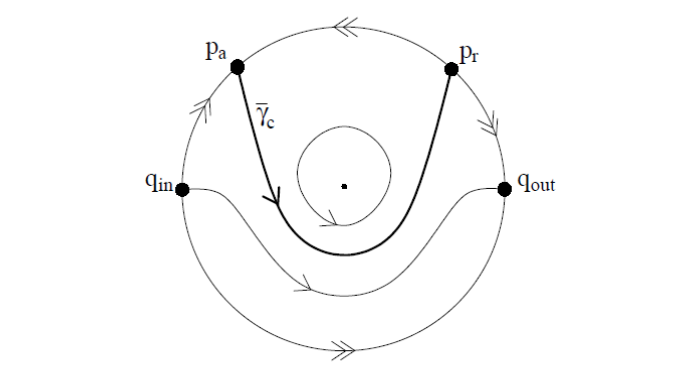
\includegraphics[height=6cm,width=10cm]{Images/CanardPointcircle}
	\caption{The flow within our canard system \citep{krupa2001}.}
	\label{fig: canard flow circle}
\end{figure}\newpage
where it is clear that our Hopf bifurcation is the periodic solution in the centre of Figure \ref{fig: canard flow circle} but we can see that below our special flow $ \bar{\gamma_c} $, our solution traverses through our equilbrium into our fast flow as we would expect in our original system.

